\فصل{پیاده‌سازی و ارزیابی}

در این پژوهش تولید سلسله فعالیت جعلی به نحوی که از دید سکو قابل تمایز با سلسله فعالیت واقعی نباشد؛ نیاز به پیاده‌سازی دقیق مدل‌سازی مطرح شده در بخش \ref{chapter:c44} و ارزیابی کامل بر اساس مدل تهدید گفته شده در بخش \ref{chapter:c42} است. در این فصل به توصیف کلی پیاده‌سازی نرم‌افزار و ارزیابی کامل آن با نمونه داده‌های متنوع بر اساس مدل تهدید سکوی بدخواه خواهیم پرداخت.

\section{پیاده‌سازی}

\section{ارزیابی}

برای ارزیابی این پژوهش میزان گمراه‌سازی سکو با تولید رخدادهای جعلی بر اساس مجموعه داده‌ای از فعالیت‌های کاربر توسط ابزار پیاده‌سازی شده اندازه‌گیری شده است. بدین منظور ابتدا هستی‌شناسی متناسب با مجموعه داده تعریف شده و پس از تولید سلسله فعالیت جعلی، ترکیب آن با سلسله فعالیت واقعی به دسته‌بند داده شده و میزان کاهش دقت آن به عنوان معیار ارزیابی در نظر گرفته شده است. این معیار نشان‌دهنده‌ قدرت راهکار پیشنهادی در گمراه‌سازی سکو است.

\subsection{مجموعه دادگان}

مجموعه داده مورد استفاده در این پژوهش مجموعه داده \lr{Orange4Home} \cite{xyz6} است که شامل تقریباً ۱۸۰ ساعت فعالیت‌های روزمره یک فرد است که به مدت ۴ هفته متوالی در روزهای کاری انجام شده است. این مجموعه داده شامل داده‌های ۲۳۶ حسگر ناهمگن است که به‌طور یکپارچه در سراسر یک آپارتمان پخش شده‌اند و ۲۰ دسته فعالیت که توسط فرد به‌طور دقیق در محل برچسب‌گذاری شده‌اند، و در مجموع ۴۹۳ نمونه از فعالیت‌ها را شامل می‌شود. این ویژگی‌ها، \lr{Orange4Home} را به یک مجموعه داده مناسب برای ارزیابی الگوریتم‌های شناسایی فعالیت، ارزیابی الگوریتم‌های پیش‌بینی فعالیت و سایر مسائل پژوهشی مرتبط با الگوریتم‌ها و خانه‌های هوشمند تبدیل می‌کند.

خانه هوشمند استفاده شده در مجموعه داده \lr{Orange4Home} شامل بخش‌های ورودی، آشپزخانه، دستشویی، پذیرایی و راه پله در طبقه همکف و راه پله، راهرو، دفتر کار، حمام و اتاق خواب در طبقه اول است که این نقشه در اشکال \ref{fig:fO4H1} و  \ref{fig:fO4H2} قابل مشاهده است.

\begin{figure}[H]
\centerline{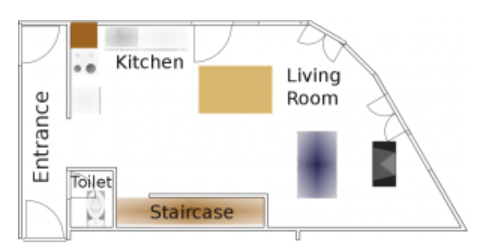
\includegraphics[width=0.8\textwidth]{figs/fO4H1.png}}
\caption{نقشه خانه مجموعه داده \lr{Orange4Home}، طبقه همکف}
\label{fig:fO4H1}
\end{figure}

\begin{figure}[H]
\centerline{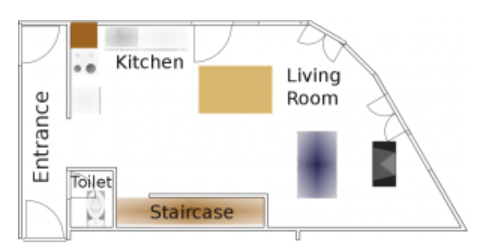
\includegraphics[width=0.8\textwidth]{figs/fO4H1.png}}
\caption{نقشه خانه مجموعه داده \lr{Orange4Home}، طبقه اول}
\label{fig:fO4H2}
\end{figure}

در هر بخش از این خانه هوشمند، حسگرهایی با انواع \پاورق{‌دودویی}{Binary}، \پاورق{‌عدد صحیح}{Integer}، \پاورق{‌عددی}{Real number} و \پاورق{‌دسته‌ای}{Categorical} وجود دارد که تعداد این حسگرها به تفکیک بخش‌های مختلف خانه هوشمند، در شکل \ref{tab:tO4H1} قابل مشاهده است (تعدادی از حسگرها در مجموعه داده \lr{Orange4Home} سراسری و برای کل خانه است).

\begin{table} [htp]
 \centering
 \caption{حسگرهای هر بخش خانه هوشمند}
 \label{tab:tO4H1}
 \begin{adjustbox}{width=\textwidth}
\begin{tabular}{|l|c|c|c|c|c|}
\hline
\textbf{محل} & \textbf{دودویی} & \textbf{عدد صحیح} & \textbf{عددی} & \textbf{دسته‌ای} & \textbf{مجموع} \\ \hline
ورودی       & 3               & 1                & 2                    & 3                    & 9             \\ \hline
آشپزخانه        & 13              & 21               & 18                   & 0                    & 52            \\ \hline
پذیرایی    & 16              & 6                & 8                    & 7                    & 37            \\ \hline
دستشویی         & 3               & 1                & 1                    & 0                    & 5             \\ \hline
راه پله      & 3               & 0                & 0                    & 0                    & 3             \\ \hline
راهرو        & 9               & 0                & 1                    & 0                    & 10            \\ \hline
حمام       & 9               & 6                & 8                    & 3                    & 26            \\ \hline
دفتر کار         & 9               & 3                & 3                    & 5                    & 20            \\ \hline
اتاق خواب        & 17              & 4                & 6                    & 7                    & 34            \\ \hline
سراسری         & 1               & 13               & 20                   & 6                    & 40            \\ \hline
\textbf{مجموع} & \textbf{83}     & \textbf{55}      & \textbf{67}          & \textbf{31}          & \textbf{236}  \\ \hline
\end{tabular}
\end{adjustbox}
\end{table}

در این مجموعه داده فعالیت‌های برچسب‌گذاری شده شامل داده‌های حسگرها می‌باشند و تمامی اطلاعات ارسالی از حسگرها بین شروع و پایان برچسب یک فعالیت است. هر فعالیت‌های برچسب‌گذاری شده متعلق به یک بخش خانه است که در ادامه لیستی از این فعالیت‌ها را داریم:

\begin{itemize}
\item \textbf{ورودی}: ورود، خروج
\item \textbf{آشپزخانه}: آماده‌سازی، آشپزی، شستن ظروف
\item \textbf{پذیرایی}: خوردن، تلویزیون دیدن، کار با رایانه
\item \textbf{دستشویی}: استفاده از دستشویی
\item \textbf{راه پله}: بالا رفتن، پایین آمدن
\item \textbf{حمام}: استفاده از روشویی، استفاده از دستشویی، حمام کردن
\item \textbf{دفتر کار}: کار با رایانه، تلویزیون دیدن
\item \textbf{اتاق خواب}: لباس عوض کردن، کتاب خواندن، خوابیدن
\item \textbf{تمامی بخش‌ها}: تمیز کردن
\end{itemize}

همانطور که گفته شد، داده‌های حسگرها بین شروع و پایان یک فعالیت برچسب‌گذاری شده ارسال می‌شوند. در مجموعه داده \lr{Orange4Home}، یک فایل \lr{csv} قرار دارد که داده حسگرها با را در خود دارد. این داده‌ها شامل زمان دقیق ارسال داده توسط حسگر، نام حسگر و مقدار ارسال شده توسط آن حسگر است که نمونه داده‌ موجود در مجموعه داده در شکل \ref{fig:fO4H3} قابل مشاهده است.

\begin{figure}[H]
\centerline{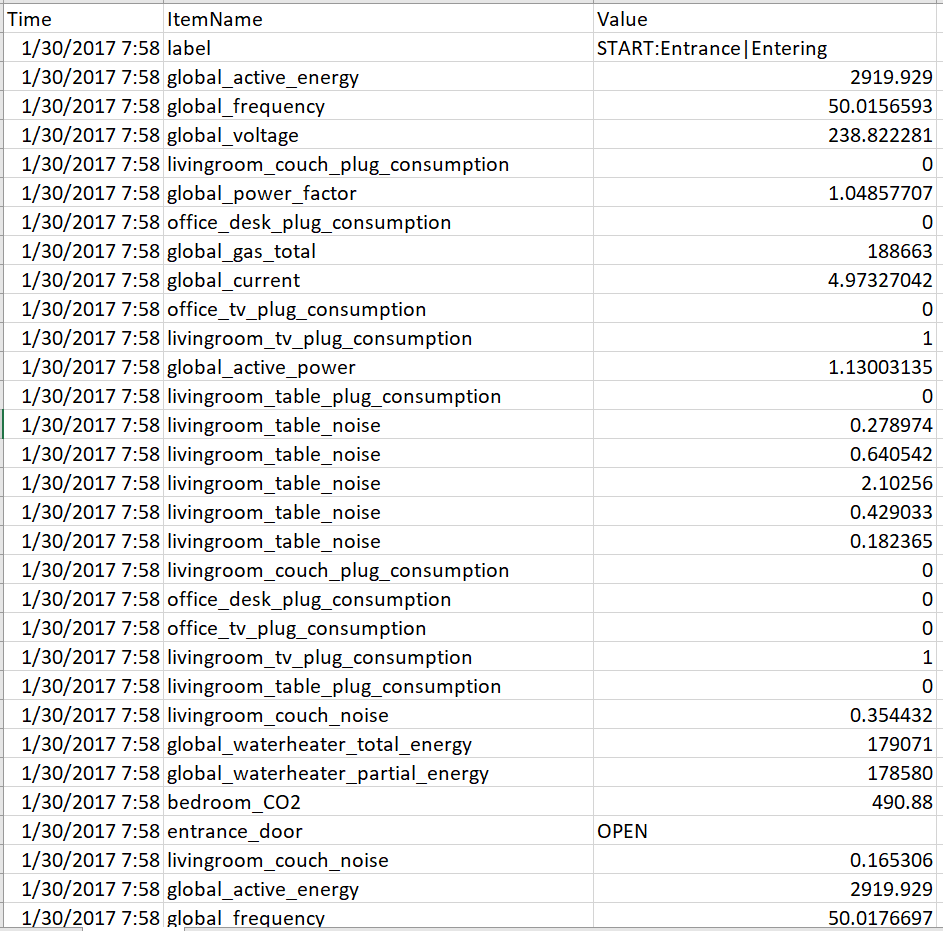
\includegraphics[width=0.8\textwidth]{figs/fO4H3.png}}
\caption{نمونه داده ارسالی از حسگرها}
\label{fig:fO4H3}
\end{figure}

\subsection{هستی‌شناسی}‌


(منطق برنامه که احتمالات حساب شد)
( رفرنس به نقشه و استفاده در آنتولوژی)
(جایگزینی لیبل با داده های سنسور ها)

\subsection{دسته‌بند}‌

\subsection{نتایج}‌

